%%%%%%%%%%%%%%%%%%%%%%%%%%%%%%%%%%%%%%%%%
% McMaster Masters/Doctoral Thesis 
% LaTeX Template
% Version 2.2 (11/23/15)
%
% This template has been downloaded from:
% http://www.LaTeXTemplates.com
% Then subsequently from http://www.overleaf.com
%
% Version 2.0 major modifications by:
% Vel (vel@latextemplates.com)
%
% Original authors:
% Steven Gunn  (http://users.ecs.soton.ac.uk/srg/softwaretools/document/templates/)
% Sunil Patel (http://www.sunilpatel.co.uk/thesis-template/)
%
% Modified to McMaster format by Benjamin Furman (contact: https://www.xenben/com; Most up 
% to date template at https://github.com/benjaminfurman/McMaster_Thesis_Template, 
% occasionally updated on Overleaf template page)
%
% License:
% CC BY-NC-SA 3.0 (http://creativecommons.org/licenses/by-nc-sa/3.0/)
%
%%%%%%%%%%%%%%%%%%%%%%%%%%%%%%%%%%%%%%%%%

%----------------------------------------------------------------------------------------
% DOCUMENT CONFIGURATIONS
%----------------------------------------------------------------------------------------

\documentclass[
11pt, % The default document font size, options: 10pt, 11pt, 12pt
oneside, % Two side (alternating margins) for binding by default, uncomment to switch to one side
english, % other languages available
singlespacing, % Single line spacing, alternatives: onehalfspacing or doublespacing
%draft, % Uncomment to enable draft mode (no pictures, no links, overfull hboxes indicated)
%nolistspacing, % If the document is onehalfspacing or doublespacing, uncomment this to set spacing in lists to single
%liststotoc, % Uncomment to add the list of figures/tables/etc to the table of contents
%toctotoc, % Uncomment to add the main table of contents to the table of contents
]{McMasterThesis} % The class file specifying the document structure


%----------------------------------------------------------------------------------------
% Import packages here
%----------------------------------------------------------------------------------------
\usepackage[utf8]{inputenc} % Required for inputting international characters
\usepackage[T1]{fontenc} % Output font encoding for international characters

\usepackage{lmodern} % could change font type by calling a different package
\usepackage{lastpage} % count pages
\usepackage{siunitx} % for scientific units (micro-liter, etc)


%----------------------------------------------------------------------------------------
% Handling Citations
%----------------------------------------------------------------------------------------
\usepackage[backend=biber,doi=false,url=false,eprint=false,firstinits=true,style=authoryear,natbib=true,sorting=ynt,maxbibnames=99,maxcitenames=2]{biblatex} % User the bibtex backend with the authoryear citation style (which resembles APA)
% can change the maxbibnames to cut long author lists to specified length followed by et al., currently set to 99.
\DeclareFieldFormat[article,inbook,incollection,inproceedings,patent,thesis,unpublished]{title}{#1\isdot} % removes quotes around title
\renewbibmacro*{volume+number+eid}{%
  \printfield{volume}%
%  \setunit*{\adddot}% DELETED
  \printfield{number}%
  \setunit{\space}%
  \printfield{eid}}
\DeclareFieldFormat[article]{number}{\mkbibparens{#1}}
%\renewcommand*{\newunitpunct}{\space} % remove period after date, but I like it. 
\renewbibmacro{in:}{\ifentrytype{article}{}{\printtext{\bibstring{in}\intitlepunct}}} % this remove the "In: Journal Name" from articles in the bibliography, which happens with the ynt 
\renewbibmacro*{note+pages}{%
    \printfield{note}%
    \setunit{,\space}% could add punctuation here for after volume
    \printfield{pages}%
    \newunit}    
\DefineBibliographyStrings{english}{% clears the pp from pages
  page = {\ifbibliography{}{\adddot}},
  pages = {\ifbibliography{}{\adddot}},
} 
\DeclareNameAlias{sortname}{last-first}
\addbibresource{Bibliography.bib} % The filename of the bibliography
\usepackage[autostyle=true]{csquotes} % Required to generate language-dependent quotes in the bibliography

% you'll have to play with the citation styles to resemble the standard in your field, or just leave them as is here. 
% or, if there is a bst file you like, just get rid of all this biblatex stuff and go back to bibtex. 

%----------------------------------------------------------------------------------------
% Collect all your header information from the chapters here, things like acronyms, custom commands, necessary packages, etc. 
%----------------------------------------------------------------------------------------
\usepackage{parskip} %this will put spaces between paragraphs
\setlength{\parindent}{15pt} % this will create and indent on all but the first paragraph of each section. 

\usepackage{acro}
\DeclareAcronym{est}{
	short = EST,
	long  = expressed sequence tags
}

\DeclareAcronym{Xl}{
	short = \textit{X.~laevis},
	long  = \textit{Xenopus~laevis}
}
\DeclareAcronym{Xg}{
	short = \textit{X.~gilli},
	long  = \textit{Xenopus~gilli}
}

\usepackage{etoolbox}
\preto\chapter{\acresetall} % resets acronyms for each chapter

\usepackage{xspace} %helps spacing with custom commands. 
\newcommand{\oddname}{{\sc SoME goOfY LonG ThiNg With an AwkWarD NAme}\xspace}


\usepackage{pgfplotstable} % a much better way to handle tables
\pgfplotsset{compat=1.12}
% \usepackage{float} % if you need to demand figure/table placement, then this will allow you to use [H], which demands a figure placement. Beware, making LaTeX do things it doesn't want may lead to oddities.  


%%%%
% LINK COLORS
% You can control the link colors at the end of the McMasterThesis.cls file. There is also a true/false option there to turn off all link colors.  
%%%%


%----------------------------------------------------------------------------------------
%	THESIS INFORMATION
%----------------------------------------------------------------------------------------

\thesistitle{Thesis Title} % Your thesis title, print it elsewhere with \ttitle
\supervisor{Dr. Jane \textsc{Smith}} % Your supervisor's name, print it elsewhere with \supname
\examiner{} % Your examiner's name, print it elsewhere with \examname
\degree{Doctor of Philosophy} % Your degree name, print it elsewhere with \degreename
\author{John \textsc{Smith}} % Your name, print it elsewhere with \authorname
\addresses{} % Your address, print it elsewhere with \addressname

\subject{Biological Sciences} % Your subject area, print it elsewhere with \subjectname
\keywords{} % Keywords for your thesis, print it elsewhere with \keywordnames
\university{\href{http://www.mcmaster.ca/}{McMaster University}} % Your university's name and URL, print it elsewhere with \univname
\department{\href{http://www.biology.mcmaster.ca/}{Department of Biology}} % Your department's name and URL, print it elsewhere with \deptname
\group{\href{http://researchgroup.university.com}{Research Group Name}} % Your research group's name and URL, print it elsewhere with \groupname
\faculty{\href{http://www.science.mcmaster.ca/}{Faculty of Science}} % Your faculty's name and URL, print it elsewhere with \facname

% this sets up hyperlinks
\hypersetup{pdftitle=\ttitle} % Set the PDF's title to your title
\hypersetup{pdfauthor=\authorname} % Set the PDF's author to your name
\hypersetup{pdfkeywords=\keywordnames} % Set the PDF's keywords to your keywords

\begin{document}

 \frontmatter % Use roman page numbering style (i, ii, iii, iv...) for the pre-content pages

\pagestyle{plain} % Default to the plain heading style until the thesis style is called for the body content

%----------------------------------------------------------------------------------------
%	Half Title (lay title)
%----------------------------------------------------------------------------------------
%\begin{halftitle} % could not get this environment working
%\vspace*{\fill}
\vspace{6cm}
\begin{center}
A short 60 character title % ideally, but it doesn't seem to matter
\end{center}
%\vspace*{\fill}
\pagenumbering{gobble} % leave this here, McMaster doesn't want this page numbered
%\end{halftitle}
\clearpage

%----------------------------------------------------------------------------------------
%	TITLE PAGE
%----------------------------------------------------------------------------------------
\pagenumbering{gobble}
\begin{center}

\vfill
\textsc{\Large \ttitle} \\

\vfill
By \authorname, \\%% -----> List prior degrees after comma  <----

 \vfill
{\large \textit{A Thesis Submitted to the School of Graduate Studies in the Partial Fulfillment of the Requirements for the Degree \degreename}}\\

\vfill
{\large \univname\, \copyright\, Copyright by \authorname\, \today}\\[4cm] % replace \today with the submission date

\end{center}


%----------------------------------------------------------------------------------------
%	Descriptive note numbered ii
%----------------------------------------------------------------------------------------
% Need to add below info
\newpage
\pagenumbering{roman} % leave to turn numbering back on
\setcounter{page}{2} % leave here to make this page numbered ii, a Grad School requirement

\noindent % stops indent on next line
\univname \\ 
\degreename\, (\the\year) \\
Hamilton, Ontario (\deptname) \\[1.5cm]
TITLE: \ttitle \\
AUTHOR: \authorname\,  %list previous degrees
(\univname)  \\
SUPERVISOR: \supname\, \\ 
NUMBER OF PAGES: \pageref{lastoffront}, \pageref{LastPage}  % put in iv and number

\clearpage

%----------------------------------------------------------------------------------------
%	Lay abstract number iii
%----------------------------------------------------------------------------------------
% not actually included in most theses, though requested by the GSA
% uncomment below lines if you want to include one
%\section*{Lay Abstract}
%\addchaptertocentry{Lay Abstract}
% Type it here
%\clearpage
%----------------------------------------------------------------------------------------
%	ABSTRACT PAGE
%----------------------------------------------------------------------------------------

\section*{\Huge Abstract} 
\addchaptertocentry{Abstract}
% Type your abstract here. 
An abstract! 
\clearpage
%----------------------------------------------------------------------------------------
%	ACKNOWLEDGEMENTS
%----------------------------------------------------------------------------------------

\begin{acknowledgements}
\addchaptertocentry{\acknowledgementname} % Add the acknowledgments to the table of contents

The acknowledgments and the people to thank go here, don't forget to include your project adviser\ldots

\end{acknowledgements}

%----------------------------------------------------------------------------------------
%	LIST OF CONTENTS/FIGURES/TABLES PAGES
%----------------------------------------------------------------------------------------

\tableofcontents % Prints the main table of contents

\listoffigures % Prints the list of figures

\listoftables % Prints the list of tables

%----------------------------------------------------------------------------------------
%	ABBREVIATIONS
%----------------------------------------------------------------------------------------
% many theses don't use this section, as it will be declared at first use and again each chapter. Uncomment these four lines to activate if you want
%\clearpage
%\section*{\Huge Acronyms}
%\addchaptertocentry{Acronyms}
%\printacronyms[name] % name without an option stops the header

%----------------------------------------------------------------------------------------
%	DECLARATION PAGE
%----------------------------------------------------------------------------------------

\begin{declaration}
\addchaptertocentry{\authorshipname}

\noindent I, \authorname, declare that this thesis titled, \enquote{\ttitle} and the work presented in it are my own. I confirm that:

\begin{itemize} 
\item List each chapter
\item and what you have done for it
\end{itemize}
 
\end{declaration}


%%%%%%%%%%%%%%%%%%%%%%%%%%%
%%%%%%%%%%%%%%%%%%%%%%%%%%%
% optional page stuff
%----------------------------------------------------------------------------------------
% can do physical constraints and symbols pages, see the original thesis example on overleaf if you want to include them at https://www.overleaf.com/latex/templates/template-for-a-masters-slash-doctoral-thesis/mkzrzktcbzfl#.VlPeicorpE4
%----------------------------------------------------------------------------------------

%----------------------------------------------------------------------------------------
%	QUOTATION PAGE
%----------------------------------------------------------------------------------------

%\vspace*{0.2\textheight}

%\noindent\enquote{\itshape Thanks to my solid academic training, today I can write hundreds of words on virtually any topic without possessing a shred of information, which is how I got a good job in journalism.}\bigbreak

%\hfill Dave Barry

%----------------------------------------------------------------------------------------
%	DEDICATION
%----------------------------------------------------------------------------------------

% \dedicatory{For/Dedicated to/To my\ldots} 

%%%%%%%%%%%%%%%%%%%%%%%%%%%
%%%%%%%%%%%%%%%%%%%%%%%%%%%
%%%%%%%%%%%%%%%%%%%%%%%%%%%



%----------------------------------------------------------------------------------------
% The following bit is just here to make sure we end up on a new page and get the total number of roman numeral
\label{lastoffront}
\clearpage
% make sure this command is on the last of your frontmatter pages, i.e. only this command, a \clearpage then \mainmatter
% should be fine without modification
%----------------------------------------------------------------------------------------

%----------------------------------------------------------------------------------------
%	THESIS CONTENT - CHAPTERS
%----------------------------------------------------------------------------------------

\mainmatter % Begin numeric (1,2,3...) page numbering

\pagestyle{thesis} % Return the page headers back to the "thesis" style

% Include the chapters of the thesis as separate files from the Chapters folder
% Example chapter, could be the introduction

\chapter{Introduction} % Main chapter title

\label{Introduction} %for referencing this chapter elsewhere, use \ref{Introduction}

\section{Introduction}

Here is where you can put a general introduction to your thesis. Just start typing away! You won't be able to render each of your chapters individually, as they are missing the preamble (the bit before the \verb+\begin{document}+). Using Overleaf makes this simple, locally (i.e. your computer) it will only be a bit more tricky. 

One of my favorite features of \LaTeX{} is the ability to put comments in your document, that are not rendered into the PDF. I leave little notes to myself all the time. You will have noticed many of these already in the document. Anything that is prefixed with a \% sign will be ignored when creating a PDF. The \% sign is a special character in \LaTeX{} (there are others too), so to print it you have to ``escape it'' as such: \verb+\%+.

Quotes too a slightly different. Use the backtick (near your escape key) for the start and an apostrophe for the end of the quote. \verb+``''+. 

\section{Citations}
When you need to cite a paper, it is simple. For a regular citation \citep{wright1932roles}. Overleaf will even give you a drop down of possible references. For multiple citations, separate with a comma \citep{wright1932roles,haldane1922sex}. For multi-author citations, the \verb+et. al+ is automatically put in.



Other citation styles are called in a similar manner.
\begin{verbatim}
\citep{} = (Wright 2015)
\citet{} = Wright (2015)
\citealt{} = Wright 2015
\citealp{} = Wright, 2015
\end{verbatim}

Citations themselves are held in the .bib file. The first line defines the key, which is used to call the citation in the text (such as ``haldane1922sex''). You can change the key to whatever. There are ways to have multiple bibliographies using various packages (bib\LaTeX{}, the one used here may support it) such as multibib and bibtopic, which would allow you to do things like print bibliographies at the end of each chapter. 

With bibtopic you would have separate .bib files and then print them within a 
\begin{verbatim}
\begin{btSect}{Chapt1.bib}
	``some print command''
\end{btSect}.
\end{verbatim}

As for the citation style at the end in the references section, I believe the GSA says go with whatever is the ``standard'' in your field. That will take a little Google-ing to get right. 

\clearpage % just here it for demonstration purposes, you do not need to specify page brakes

One nice feature is creating short names for species, and other acronyms. In the preamble of the main text, you can define these acronyms. They would look something like:
\begin{verbatim}
\DeclareAcronym{est}{
	short = EST,
	long  = expressed sequence tags
}

\DeclareAcronym{Xl}{
	short = \textit{X.~laevis},
	long  = \textit{Xenopus~laevis}
}
\DeclareAcronym{Xg}{
	short = \textit{X.~gilli},
	long  = \textit{Xenopus~gilli}
}
\end{verbatim}

These could allow you to write \ac{est} and \acl{Xl}, which will bring the full name the first time, then the short form all other times. So we can call them again \ac{est} and \ac{Xl}. We can even pluralize them \acp{est}, if necessary. For species names, I generally use \verb+\acl+ the first time, then \verb+\ac+ the other times. If I mention another species with the same genus name, such as \acs{Xg}, I use \verb+\acs+ the first time (so that I do not repeat the genera name) and all other time use \verb+\ac+. There are a lot of options, beyond ``short'' and ``long'', if you need more complicated things with your acronyms. 

Another option for odd names is to define a custom command. This is set with
\begin{verbatim}
\newcommand{\oddname}{{\sc SoME goOfY LonG ThiNg With an AwkWarD 
                                                NAme}\xspace}
\end{verbatim}

Then called however you defined it: \oddname.

\section{Handling a supplement}

You could drop supplemental sections directly in this chapter \TeX{} file. There are fancy ways to have it as a separate \TeX{} file, but that can get complicated with a book style document. 

Alternatively, you could put it as an Appendix at the end of your thesis. 

We can then reference the Figure in the supplement (Fig.\,\ref{Another_fig}; see Chapter \ref{nextChapt} for handling figures). 










      
% remember to set these at the start of each chapter
\chapter{The Next Chapter} 
\label{nextChapt} 

%%%%%%%%%%%%%%%%%%


\section{What About Figures}

Figures are dead easy to call. Just call them from within a Figure environment.

\begin{figure}[h] % put figure roughly here, will float though
	\centering
	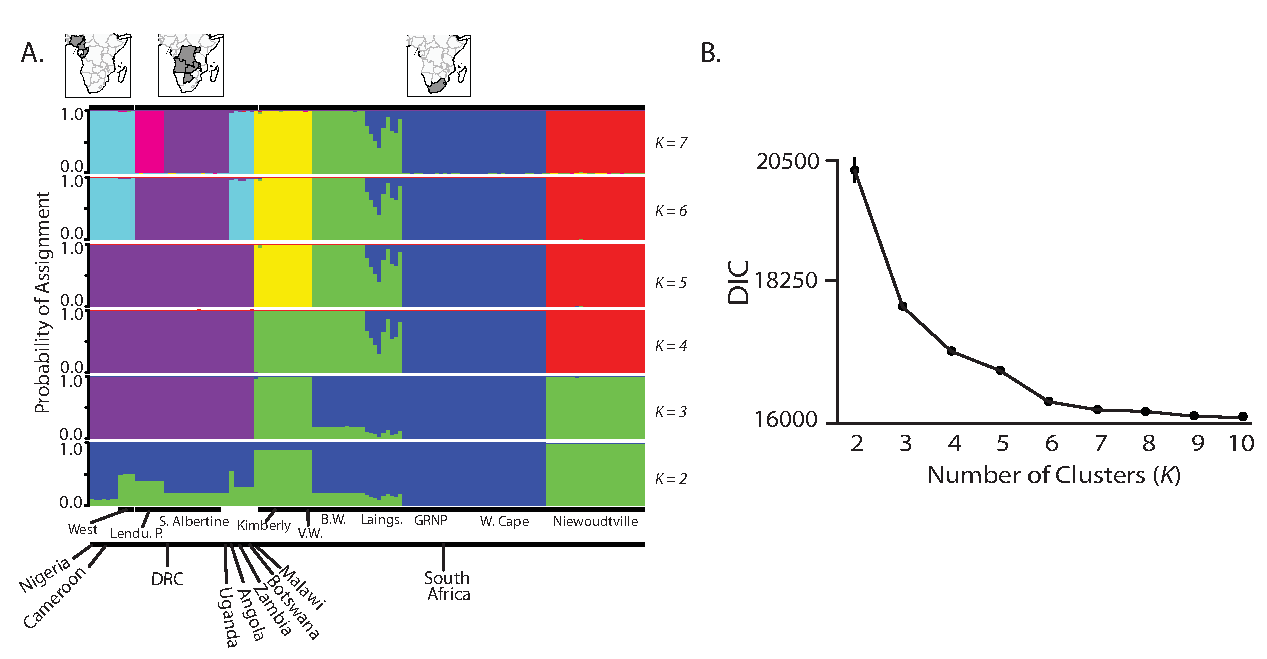
\includegraphics[scale=0.6]{Figs/Fig3_TESS_full_round2.pdf}
    \caption[Admixture]{Genetic structure of populations\ldots}
    \label{tess_analysis}
\end{figure}

And now, I do not need to remember the figure number. All I do is refer to the figure label that I gave it (Fig.\,\ref{tess_analysis}).


As for my next figure, \LaTeX will automatically do the numbering. It will also attach the chapter number to the figure.



\begin{figure}[h!] % put figure roughly here, will float though, h! will strongly suggest where to put it.
	\centering
	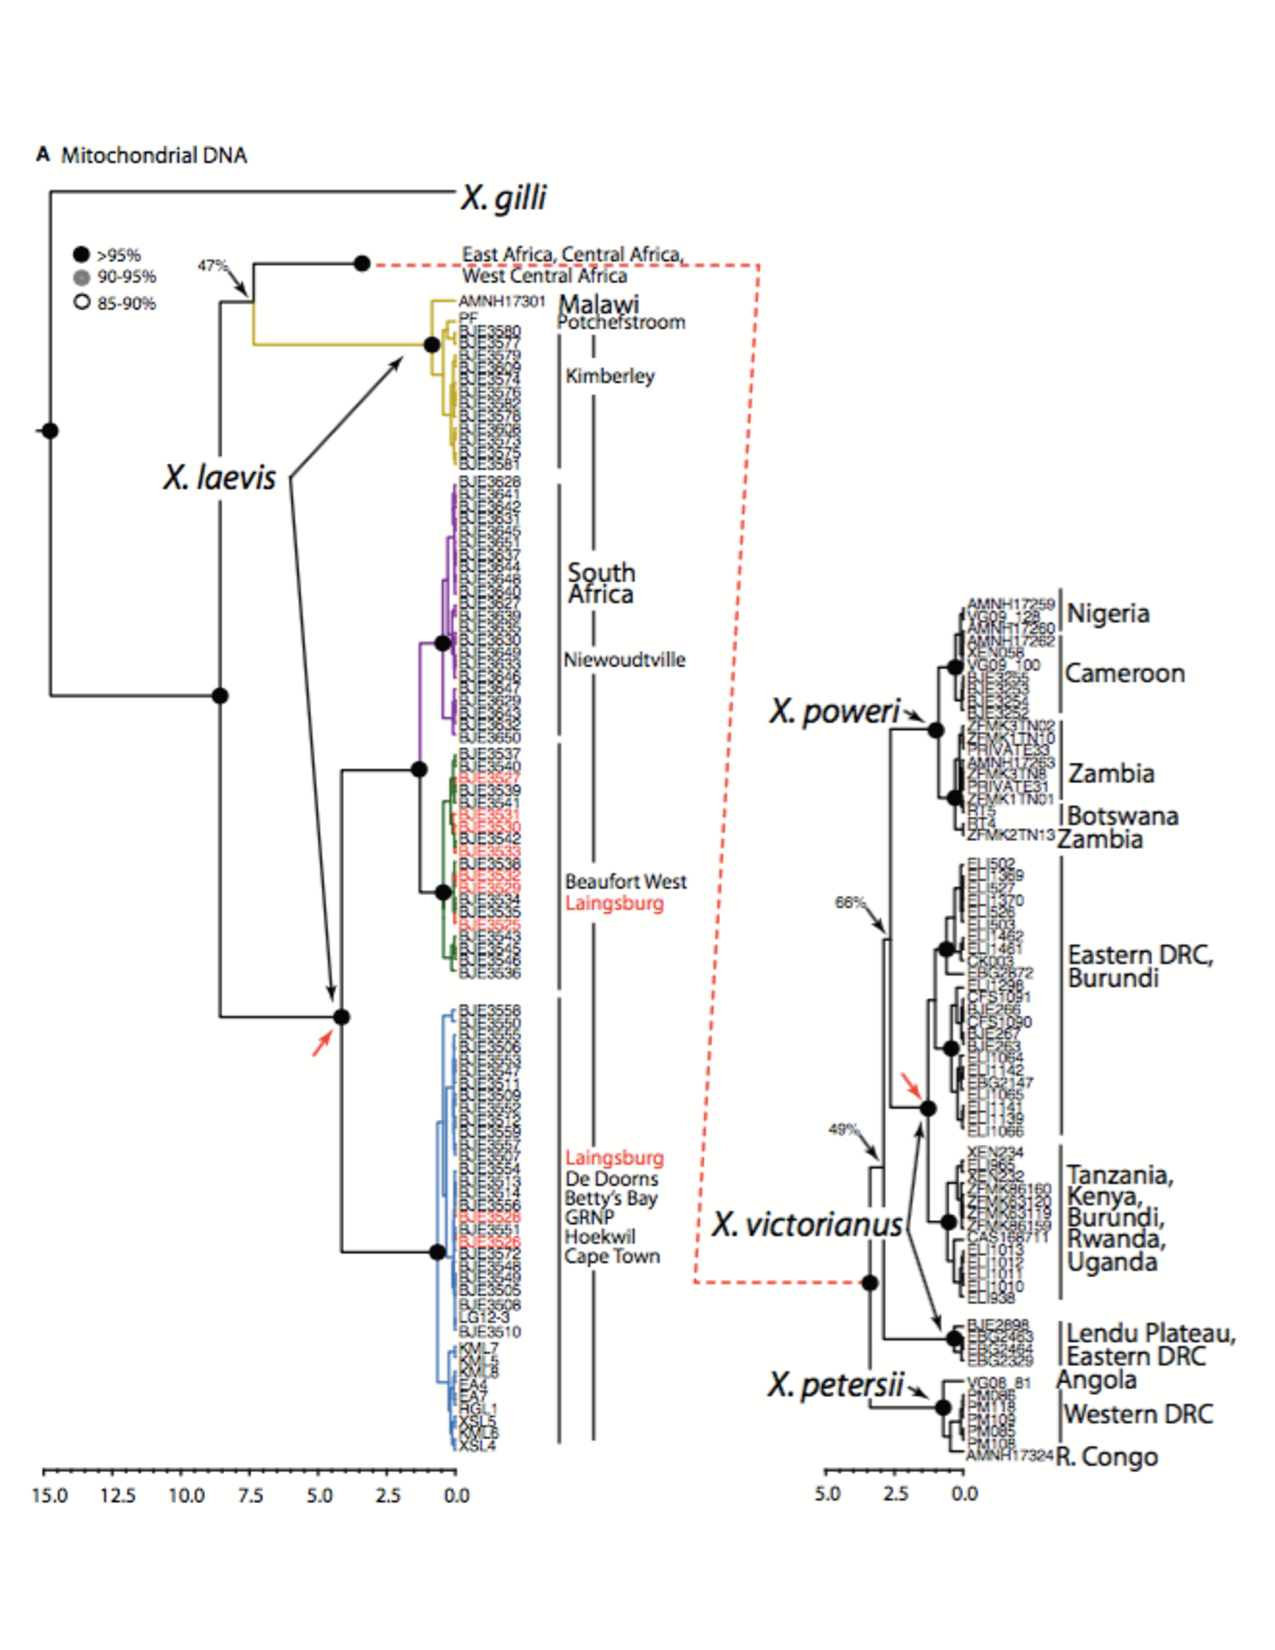
\includegraphics[scale=0.6]{Figs/Tree_Fig.pdf}
    \caption[Tree]{A tree of \ac{mtdna}\ldots}
    \label{Tree}
\end{figure}

Then I will call it same as before (Fig.\,\ref{Tree}). As you can see, it was placed on the next page, as \LaTeX thought that was best, given its size. Figures will float around, but you will never have to worry about numbering. You may notice the \verb+\,+ that just puts in a small space after the Fig. period. \emph{Remember, scalar rendered (Illustrator, Inkscape, R) graphics will not distort! Avoid powerpoint/excel at all costs}. I took a screen shot, which is why these trees look like crap. 

Did you notice that the table of contents/list of figures was all automatically updated too\ldots\.pretty neat. 


\section{Tables -- how to}

\subsection{Typing in Tables}
Small to medium tables I would suggest just typing it in to the \TeX file (see Table \ref{simpleTable} below). There are also packages to create \LaTeX tables (such as xtable in R) and packages to read in csv/tab files, like you read in figures. There are ways to make multi-column and multi-row values in tables; you will have to Google it (it is not hard to do). The \verb+\usepackage{multirow}+ will allow you to do multirow values. The command \verb+\multicolumn{}{}{}+ is already available. 

\begin{table}[h]
\centering
\caption[Simple table]{A simple typed in table. Note the special lines used in the table. Yes, typography rules call for different thickness of lines. The command \\hline will put in just a regular horizontal line}
\label{simpleTable}
\begin{tabular}{c|ccc} 
\toprule
col1 & col2 & col3 & col4 \\
\midrule
1 & 2 & 3 & 4 \\
1 & 2 & \multicolumn{2}{c}{3} \\
\bottomrule
\end{tabular}
\end{table}



% reading in a csv file
\subsection{Reading in CSV table}

You can copy and paste the information into \LaTeX to keep things together, but it has to be dropped into the preamble in the main tex. Or you can call in the data file (Table \ref{csv_readin}).

Using \verb+\usepackage{pgfplotstable}+ is the package to use.

\begin{table}[h]
\centering
\caption[Normal size table]{Reading in a table}
\label{csv_readin}
\pgfplotstabletypesetfile[col sep=comma,every last row/.style={after row=\bottomrule},every head row/.style={before row={\toprule}, after row={\midrule}}]{Tables/Suppl_Table_1.csv}
\end{table}

If tables do not fit, you can shrink them by wrapping in a box or shrinking text (Table \ref{csv_readin_small}).

\begin{table}[h]
\tiny % add text size command 
\centering
\caption[Tiny table]{Reading in a table}
\label{csv_readin_small}
\pgfplotstabletypesetfile[col sep=comma,every last row/.style={after row=\bottomrule},every head row/.style={before row={\toprule}, after row={\midrule}}]{Tables/Suppl_Table_1.csv}
\end{table}

And it is just as easy to rotate tables, and only a little bit difficult to do multi-page rotated tables, any what ever else you want, but packages exist to handle it. 

\section{Clickable Fig/Table refs}

One of the really nice thing about \LaTeX is that the Figure and Table references in text are clickable and will take you to whatever is being referenced (click this number -- Fig. \ref{Another_tree}). There are also commands you can put in to then return, but these are a bit more tricky. 

The same is true for your section headings and the entire table of contents and lists of figures/tables. Additionally, anything that has been given a \verb+\label{}+, when called with a \verb+\ref{}+ will be clickable. 











 

%----------------------------------------------------------------------------------------
%	THESIS CONTENT - APPENDICES
%----------------------------------------------------------------------------------------

\appendix % Cue to tell LaTeX that the following "chapters" are Appendices

% Include the appendices of the thesis as separate files from the Appendices folder
\chapter{Chapter 1 Supplement} % Main appendix title

\label{Supp_chap1} % Change X to a consecutive letter; for referencing this appendix elsewhere, use \ref{AppendixX}


Here is the supplemental file for chapter 1, as an alternative to including it in the main \TeX for chapter 1. This allows the figures/table to be numbered in a different way and for the section to be listed in the table of contents differently. 


\begin{figure}[h] % put figure roughly here, will float though
	\centering
	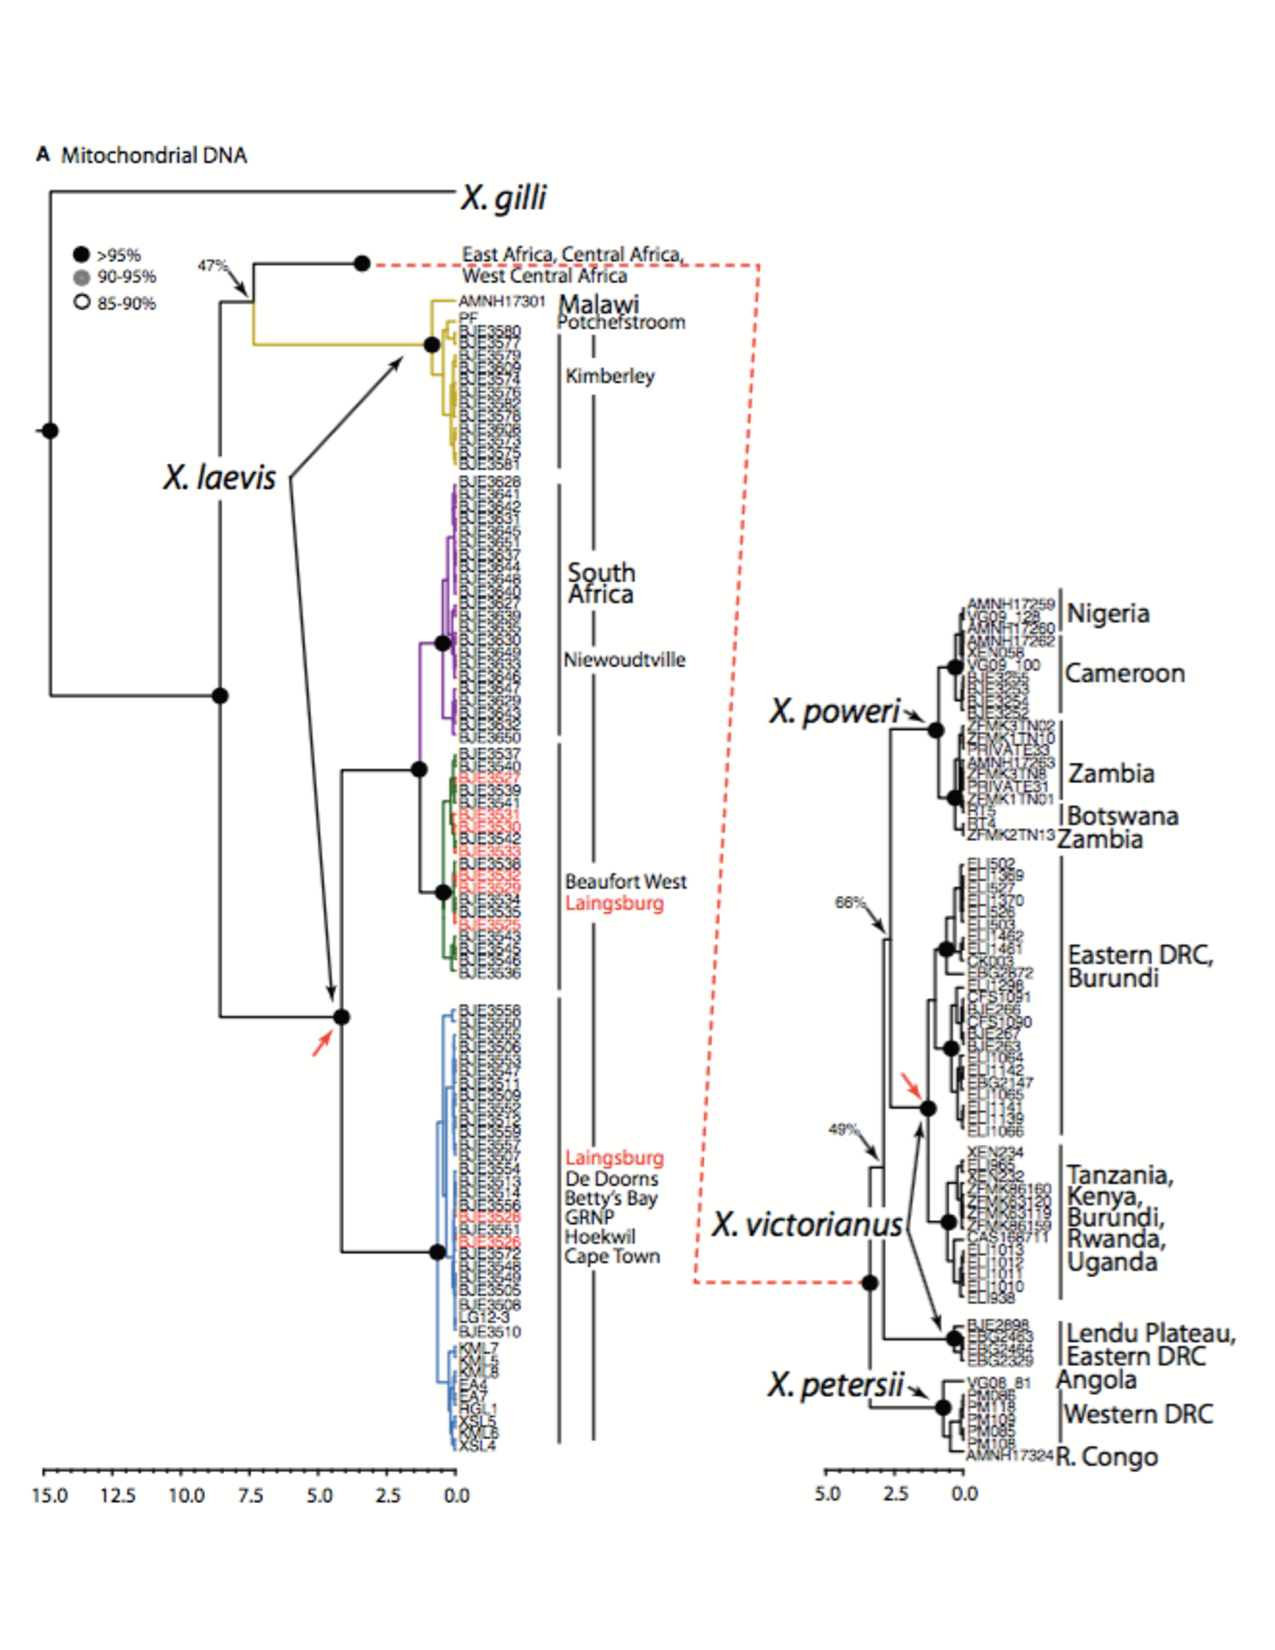
\includegraphics[scale=0.6]{Figs/Tree_Fig.pdf}
    \caption[Same Tree]{Same tree as before, but in the appendix!}
    \label{Another_tree}
\end{figure}



%----------------------------------------------------------------------------------------
%	BIBLIOGRAPHY
%----------------------------------------------------------------------------------------

\printbibliography[heading=bibintoc]

%----------------------------------------------------------------------------------------

\end{document}